\documentclass[conference, usletter]{IEEEtran}
\IEEEoverridecommandlockouts
% The preceding line is only needed to identify funding in the first footnote. If that is unneeded, please comment it out.
\usepackage{cite}
\usepackage{algorithmic}
\usepackage{graphicx}
\usepackage{textcomp}
\usepackage{amsmath}
\usepackage[sc]{mathpazo}
\usepackage{datetime}
\usepackage{graphicx, wrapfig, subcaption, setspace, booktabs}
\usepackage[T1]{fontenc}
\usepackage{fourier}
\usepackage{url, lipsum}
\usepackage{hyperref,bookmark}
\usepackage[T1]{fontenc}
\usepackage{amssymb}
\usepackage{makecell, multirow, tabularx}
\usepackage{listings}
\usepackage[ruled,linesnumbered,vlined]{algorithm2e}

\usepackage{float}
\usepackage{nomencl}
\usepackage{ifthen}

\renewcommand{\nomgroup}[1]{%
	\ifthenelse{\equal{#1}{P}}{\item[\textbf{Parameters}]}{%
		\ifthenelse{\equal{#1}{V}}{\item[\textbf{Variables \\}]}}
}
\makenomenclature
\def\BibTeX{{\rm B\kern-.05em{\sc i\kern-.025em b}\kern-.08em
    T\kern-.1667em\lower.7ex\hbox{E}\kern-.125emX}}
\begin{document}

\title{CO\textsubscript{2} and Cost Impact Analysis of a Microgrid  with Electric Vehicle Charging Infrastructure: a Case Study in Southern California}

\author{
	\IEEEauthorblockN{Luis Fernando Enriquez-Contreras\IEEEauthorrefmark{1}\IEEEauthorrefmark{2}, Matthew Barth\IEEEauthorrefmark{1}\IEEEauthorrefmark{2}, Sadrul Ula\IEEEauthorrefmark{2}}
	\IEEEauthorblockA{\IEEEauthorrefmark{1}\textit{Department of Electrical  and Computer Engineering} \\
		\textit{University of California, Riverside}\\
				Riverside, United States of America \\
				lenri001@ucr.edu, barth@ece.ucr.edu}
	\IEEEauthorblockA{\IEEEauthorrefmark{2}\textit{College of Engineering, Center for Environmental Research \& Technology} \\
		\textit{University of California, Riverside}\\
				Riverside, United States of America \\
				lenri001@ucr.edu, barth@ece.ucr.edu, sula@cert.ucr.edu}
}
\maketitle

\begin{abstract}
	As a part of  an innovative Intelligent Transportation System (ITS), this paper investigates the effectiveness of transportation-based microgrid configurations in reducing carbon dioxide (CO\textsubscript{2}) emissions and electricity costs. A case study at the University of California, Riverside (UCR) utilizes high-resolution California Independent System Operator (CAISO) CO\textsubscript{2}  emission data to assess the environmental impact of each microgrid configuration. It also compares electricity costs to determine potential consumer savings. The results demonstrate that a load-following transportation microgrid strategy can significantly reduce CO\textsubscript{2}  emissions (67\%–84\%) and achieve annual cost savings of approximately \$24,000, even when accounting for the additional demand from daily electric vehicle (EV) charging at the building. However, battery sizing is crucial for cost-effectiveness, as load-following exhibits diminishing returns. Doubling battery capacity may yield negligible reductions in electricity costs and CO\textsubscript{2}  emissions after exceeding certain threshold. This emphasizes the importance of optimizing battery capacity to achieve a balance between cost and environmental impact. The study further reveals that Level 2 chargers in a commercial building generally have minimal impact on building demand and energy charges. Conversely, a single Level 3 DC fast charger has a more significant impact, requiring increased solar and battery storage capacity for further cost reduction. %The new net metering rates incentivize users to reduce grid dependence and utilize more local clean energy sources for EV charging.
\end{abstract}
\begin{IEEEkeywords}
	Infrastructure for Charging, Communication and Controls, Energy Storage and Control Systems, Electric Vehicles %load-following, modelica, distributed energy resources, greenhouse gas analysis, transportation electrification  
\end{IEEEkeywords}
\section{Introduction}
\subsection{Background}
California is committed to reducing greenhouse gas emissions (GHG) through various approaches, particularly in the two largest sectors: transportation and electricity generation. In California, electric vehicles (EVs) accounted for 25.4\% of Q2 2023 vehicle sales \cite{ev_sale_percentage}, and the state will ban the sale of internal combustion engine vehicles by 2035 \cite{ice_ban}. Concurrently, California is expanding the number of EV charging stations in the state, with 13,844 Level 2 and 1,924 Level 3 stations \cite{ev_stations_CA} as of November 2023. EV technology has advanced, and new EVs can typically charge up to 80\% in 20-60 minutes \cite{ev_stats}. This is made possible by Level 3 DC fast charging, which can deliver up to 350 kilowatts (kW), compared to Level 2 charging, which is limited to 19 kW \cite{ev_stats}. While this reduced charging time has increased the attractiveness of EVs, it also poses a challenge for the owners of these chargers, as they can quickly demand a large amount of electricity demand. As California strives to increase the share of clean energy in its electricity mix, it also needs to reduce the CO\textsubscript{2} emissions from transportation by promoting electrification. This leads to two conundrums: how will California provide enough capacity for electrified transportation, and how clean is the grid that minimizes the emissions associated with battery electric vehicles? One method to alleviate the pressure on the grid is to localize electricity production and EV charging using microgrids. A microgrid is defined by the Department of Energy (DOE) and the Institute of Electrical and Electronics Engineers (IEEE) as: "a group of interconnected loads and distributed energy resources within clearly defined electrical boundaries that acts as a single controllable entity with respect to the grid. A microgrid can connect and disconnect from the grid to enable it to operate in both grid-connected or island-mode." \cite{microgrid_def} \cite{microgrid_def_ieee}. As microgrids and EV chargers become more widespread, it is essential to study the economic and environmental impacts of EV charging, especially fast charging, and the effect of microgrids on that impact. EV charging differs from typical building loads, as it can rapidly ramp up to high levels at random intervals based on human behavior, i.e., when they plug in. An outlier event where multiple people charge simultaneously can cause a significant peak in the load. 

This research holds significant implications for the advancement of intelligent transportation systems, as it aims to address the economic needs of EV charging infrastructure owners and determine the optimal configuration that benefits both EV owners and the environment by minimizing GHG emissions. This paper delves into the impacts of  Level 2 and Level 3 charging infrastructure on the behavior of microgrids, associated electricity costs, and CO\textsubscript{2} emissions within the context of Southern California. The simulations are conducted using OpenModelica \cite{ModelicaLanguage}, a dynamic modeling and simulation environment. This study distinguishes itself from previous research in many ways, including employing a higher time resolution for calculating CO\textsubscript{2} emissions, capturing data every 15 minutes.
%		This work is crucial for intelligent transportation systems since new EVs should also benefit those who own EV charging infrastructure. Understanding the economic needs of EV charger owners and what setup can be beneficial for them and EV owners and best reduce greenhouse gas emissions from the environment is a topic that needs to be further investigated. This paper analyzes the impacts of transportation microgrids with Level 2 and Level 3 charging on the behavior of microgrids and the associated electric costs and CO\textsubscript{2} emissions in southern California. The simulation is run in OpenModelica, a dynamic modeling and simulation environment. This paper also uses higher time resolution data than most studies to calculate the CO\textsubscript{2} emissions every 15 minutes.
\subsection{Literature Review}
Transportation microgrids have gained significant traction in recent years due to the growing demand for transportation electrification. These microgrids, which combine distributed energy resources (DERs) and energy storage systems with electric vehicle (EV) charging infrastructure, offer a promising solution for integrating EVs into the power grid while minimizing environmental impact. Previous studies have investigated the economic viability of transportation microgrids, primarily focusing on energy charges associated with EV charging. However, demand charges, which reflect the peak demand imposed on the grid, need to be addressed. This inclusion is crucial for fast charging stations, which draw significant power during peak periods. A more comprehensive approach to economic analysis should consider energy and demand charges, providing a more accurate assessment of the overall cost of operating a transportation microgrid. Research has addressed the impact of EV charging demand on transportation microgrids, often focusing on low-demand Level 2 charging. However, the increasing deployment of high-demand Level 3 charging requires a more nuanced understanding of its implications. Studies should incorporate a mix of Level 2 and Level 3 charging scenarios to accurately assess the impact of EV charging demand on microgrid operation and economics. Assessment of the GHG emissions associated with transportation-microgrids is often simplified by using average CO\textsubscript{2} emissions from an area's electricity production. This approach fails to capture the variations in CO\textsubscript{2} emissions throughout the day, which can significantly affect the environmental impact of EV charging. More sophisticated GHG emission calculations should consider the time-varying nature of CO\textsubscript{2} emissions, providing a more accurate representation of the environmental impact of transportation microgrids. 

Several studies have investigated the performance of electric vehicle charging stations (EVCS) under varying conditions. Reference \cite{himabindu2021analysis} is developing a demand and stochastic model for EVCS, followed by a techno-economic assessment and an environmental impact analysis. They concluded that the optimal configuration and investment costs of EVCS with solar integration are highly dependent on feed-in tariffs and solar irradiation levels. However, their CO\textsubscript{2} emission calculations were based on annual averages and did not account for intraday variations. They only considered energy charges, omitting demand charges in their economic analysis. Reference \cite{yoon2017economic} proposed a control algorithm for EVCS that can minimize charging time, minimize costs, or maximize renewable energy use depending on the scenario. They modeled charging loads using a uniform distribution during peak demand periods, assuming only Level 2 charging at 3.3 kW and excluding Level 3 charging. Reference \cite{purvins2018electric} proposed an EV charging model that shifts charging events from peak demand periods to off-peak times. They found that their current method had limited impact on peak load shaving and that solar production surplus may only sometimes be diverted to EVs due to their low availability during those times. Their dataset was limited to one week, involving four EVs in a system with ten buildings. Reference \cite{Khemir} ran multiple scenarios with different self-consumption rates, comparing scenarios first and then calculating emissions for each. Their CO\textsubscript{2} emission calculations were based on whole-life-cycle CO\textsubscript{2} emissions without high time resolution. Reference \cite{huang2023multi} employed the Non-dominated Sorting Genetic Algorithm-II (NSGA-II) to analyze four different responses with EV penetration rates of 0\%, 10\%, 20\%, and 30\% using a Monte Carlo load profile. They achieved remarkable results but did not elaborate on their CO\textsubscript{2} calculations or provide a detailed analysis of the specific impacts of Level 2 versus Level 3 charging. Reference \cite{tan2020multi} analyzed IEEE 9 and 14 bus systems, forecasting EV loads one day ahead. They utilized multiple microgrids to balance out EV charging within the system, employing a multi-objective energy management approach for optimizing microgrid operation. The forecasted EV loads did not have sudden high-demand events nor level 3 charging, which makes the forecasting model challenging to implement. A similar problem arises in Reference \cite{PV_EV_Charging_Station}, which performs a techno-economic analysis of PV EVCS with BESS. Their analysis also varies battery size to find the net present values that would make the project economically viable. However, it is limited to only one Level 2 electric vehicle. While their cost experiment spans the course of a year, it only uses the total energy for the year, which is multiplied by an annual CO\textsubscript{2} emissions rate.
%  		In  \cite{himabindu2021analysis},   Electric Vehicle Charging Stations (EVCS) are analyzed under different solar irradiation conditions.   The study develops a demand and stochastic model, then performs a techno-economic assessment and analyzes the environmental impact of EVCS.  The authors conclude that EVCS with solar's optimal configuration  and investment costs are highly dependent on feed-in tariffs and  the solar irradiation of the area. The  CO\textsubscript{2} emissions were calculated on a per year basis, and do not deal with the variations of  CO\textsubscript{2} emissions within a single day.  Also, only energy charges were calculated with no demand costs calculations. \citen{yoon2017economic},  proposes a control algorithm is proposed that in different scenarios can minimize charging time or costs or maximize renewable energy use. The authors used a uniform distribution during peak times  to model the charging loads, with only Level 2 charging at 3.3 kW and no Level 3 charging. An EV charging model is proposed in \cite{purvins2018electric},  that load shifts charging events from high peak times to low peak times.  The authors found their current method does little to reduce peak load shaving, and solar production surplus may not be necessarily shifted to EVs due to their low availability at the time.  The dataset was limited to one week ], with four EVs in a system with 10 buildings.  In \cite{Khemir}, the authors run multiple scenarios with different self consumption rates, first comparing scenarios and then calculating emissions for each scenario.. The CO\textsubscript{2} emissions are calculated from whole life-cycle CO \textsubscript{2}  emissions without a high time resolution.  \cite{huang2023multi} uses the Non-dominated Sorting Genetic Algorithm-
%  		II (NSGA-II) to analyze 4 different responses with 0 \% 10 \% 20 \% 30\%  EV penetration and a Monte Carlo load profile.  Results were remarkable, however CO\textsubscript{2} calculations were not explained. and the specific impacts of  Level 2 vs Level 3 charging were not shown.  \cite{tan2020multi} analyzes IEEE  9 and 14 nodes  that forecast the EV loads one day ahead.  The author use multiple microgrids to balance out EV charging within the system.  Multi-objective energy management of multiple microgrids is used to orchestrate the operation.
%  		
%  		This paper's analyzes the impacts different Level 2 and Level 3 charging have on the behavior of microgrids and the associated electric costs and CO\textsubscript{2} emissions in southern California. The simulation is run in open Modelica rather than being a purely calculated model. This paper also uses a higher time resolution data than most to calculate the CO\textsubscript{2} emissions every 15 minutes.
%    \subsection{Peak Shaving Strategy}
%%       		Peak shaving is a standard method for reducing high-demand charges. Since demand charges are based on only the maximum value over the entire month, we assume the consumer wants to minimize the demand charges as much as possible. Energy charges is the charge for the amount of energy used throughout the month, as opposed to demand charges this is a summation instead of a maximum value. Our algorithm is based solely on cost savings for a typical microgrid. During peak-shaving, the algorithm looks at the amount of power being imported, if there is enough energy, and if the batteries can mitigate a fraction of that or the total amount.  
%		Peak shaving is a widely adopted strategy for mitigating high-demand charges. As demand charges are solely determined by the maximum power consumption over an entire billing period, it is assumed that consumers seek to minimize these charges to the greatest extent feasible. Energy charges, on the other hand, represent the cost associated with the total energy consumed during the billing period and are calculated as a summation rather than a maximum value. The proposed algorithm is designed to optimize cost savings managing demand and energy charges using a typical microgrid. During peak-shaving periods, the algorithm assesses the imported power, evaluates the availability of sufficient energy, and determines whether batteries can mitigate a portion or the entirety of the imported power demand.
 \subsection{CO\textsubscript{2} Emissions}
 Our microgrid's solar production, shown in Fig. \ref{fig:powersystemsetupfull}, largely overlaps with the local solar energy production within the larger grid. With a Battery Energy Storage System (BESS), we can utilize renewable energy during peak times and at night. In this scenario, the control algorithm is optimized to minimize cost for the consumer. However, we want to see how low-price EV charging aligns with actual CO\textsubscript{2} emission outputs. While the microgrid does not produce any direct CO\textsubscript{2} emissions, CO\textsubscript{2} emissions are attributed to the microgrid when it pulls power from the main power grid. The simulation uses emission output calculations from the California Independent System Operator (CAISO) for each time interval as a sum of all the powerplant CO\textsubscript{2} emissions (imports, natural gas, biogas, biomass, geothermal, coal) $\frac{\textsubscript{m}TON\textsubscript{CO\textsubscript{2}}}{hour}$. The CO\textsubscript{2} emissions output is divided by the amount of power produced (solar, wind, geothermal, biomass, biogas, small hydro, grid batteries, large hydro, imports, nuclear, coal ) in MW, which gives us an emissions rate of $\frac{\frac{\textsubscript{m}TON\textsubscript{CO\textsubscript{2}}}{hour}}{W}$. This is multiplied by 15-minute data kW and a multiplier. The multiplier of  $\frac{1}{4000}$ converts kW into W and addresses the four 15-minute periods in an hour. CAISO gives us an estimate of the amount of CO\textsubscript{2} emissions in \textsubscript{m}TON\textsubscript{CO\textsubscript{2}} for every 15 minutes that is summed to give us the total for the entire period. This method is similar to the one used in \cite{garrido2021dynamic}. The CO\textsubscript{2} calculations use 15-minute intervals to align with the time intervals used for billing and demand cost by electric utilities. When the microgrid does not pull power from the grid or is sending power, the CO\textsubscript{2} emissions are assumed to be zero since we are using renewable solar energy.
 \section{Simulation in OpenModelica}
 OpenModelica is an open-source implementation of the Modelica programming language \cite{OpenModelica}. Modelica is a programming language that is designed for dynamic systems simulation \cite{ModelicaLanguage}. OMEdit is the GUI interface for OpenModelica, allowing the user to draw a system for simulation \cite{OMEdit}. The microgrid scenarios are simulated in OpenModelica using the Modelica Buildings library. Lawrence Berkeley National Laboratory created the Modelica Buildings library for building and district energy and control systems \cite{ModelicaBuildingsLibrary}.
 Further, its capability for energy storage systems, bi-directional inverter, solar, and HVAC modeling make it ideal for a microgrid simulation setup. This allows us to create scenarios that do not currently exist in our microgrid, shown in Fig. \ref{fig:powersystemsetupfull}, for example, running a month with solar with the same load or running the BESS control algorithm for different electric rates. The power circuits are three-phase balanced circuits. The simulation of our case study microgrid is the grid connected to the building netload. The model's net load is broken down into solar power, HVAC loads, regular building loads, electric vehicle chargers, and the BESS, as shown in Fig.\ref{fig:powersystemsetupfull}.
 \begin{figure*}
 	\centering
 	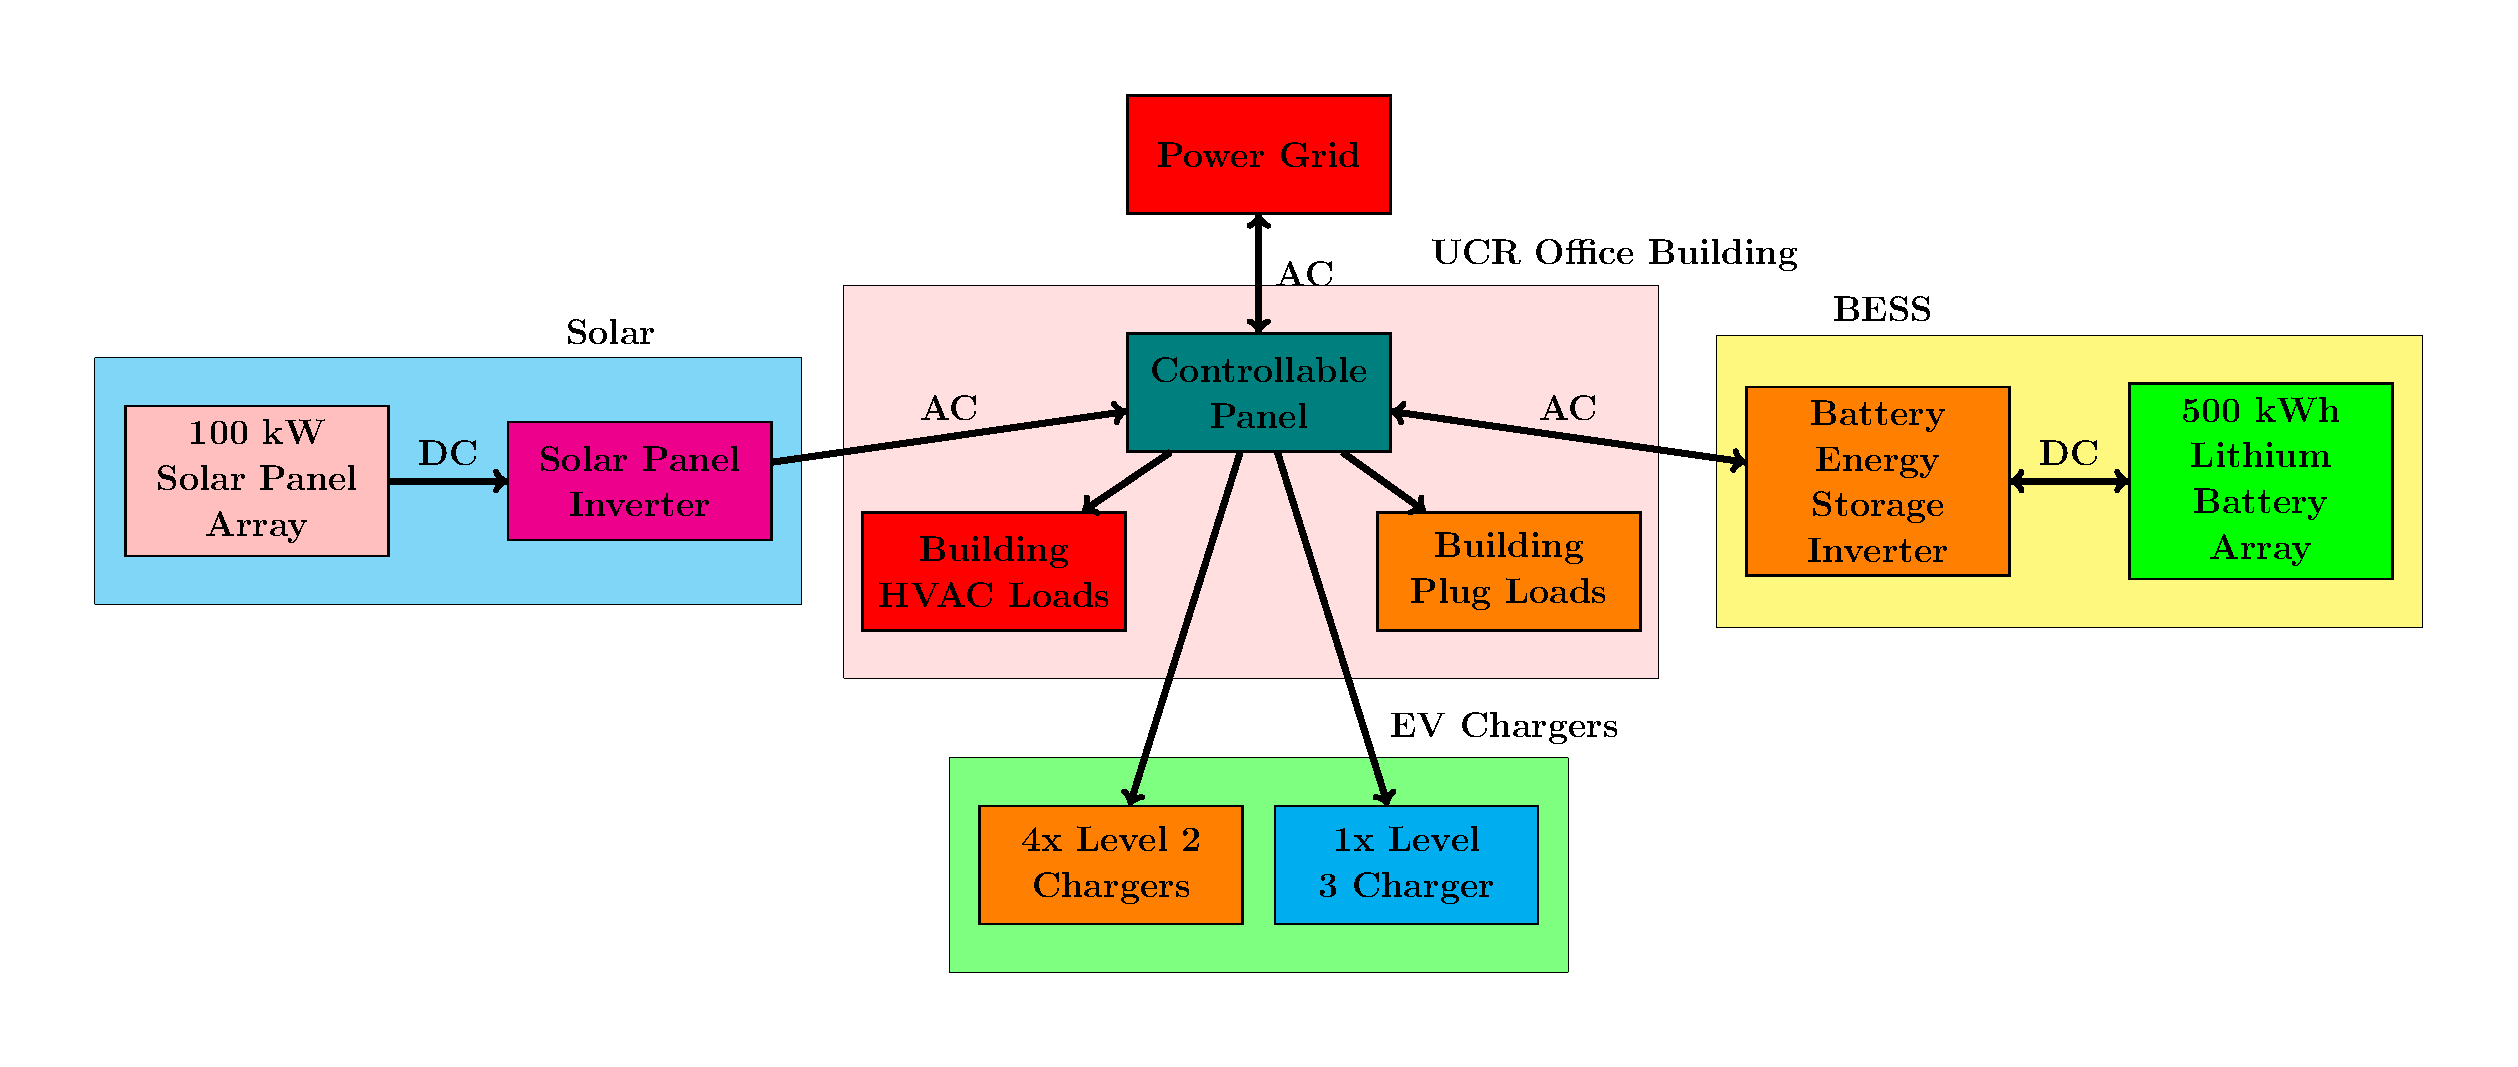
\includegraphics[width=\linewidth]{Fig/power_system_setup_modelica_large}
 	\caption{\footnotesize Microgrid Architecture of our Case Study Example BESS: Battery Energy Storage System}
 	\label{fig:powersystemsetupfull}
 \end{figure*}
	\subsection{Validation}
A year of real-world data was used to validate the $P_G $ output to ensure that our model accurately portrays our real-world system. $P_G$ is the power the microgrid sends or consumes from the grid. The actual data was compared to the simulated with a correlation coefficient of  $\approx$ 0.965087 as shown in Figure \ref{fig:ucr15minutedatamar012022tomar012023}. 
\begin{figure}
	\centering
	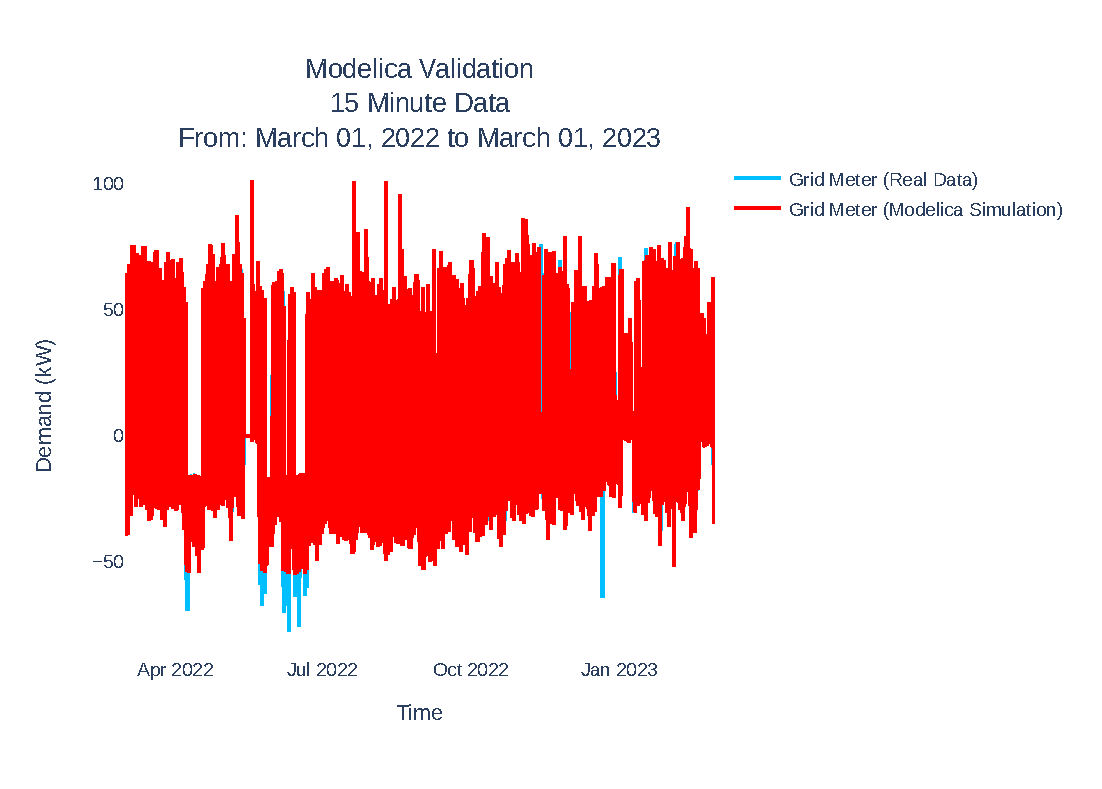
\includegraphics[width=0.9\linewidth]{Fig/ucr_15_Minute_Data_Mar_01_2022_to_Mar_01_2023}
	\caption{\footnotesize Whole Year Validation of the Microgrid Architecture in OpenModelica. The bright blue and red are the real data and simulated data, respectively. The dark red is the overlap between real and simulated data.} %the two, which is the majority of the plot. This is expected since real and simulated data should be similar, and the simulated power flow calculations should accurately represent the microgrid.}
\label{fig:ucr15minutedatamar012022tomar012023}
\end{figure}
\subsection{Solar Generation and Building Loads}
The solar power in our model is based on historical solar data from a 100 kW photovoltaic (PV) array. The HVAC loads and the regular building loads are represented separately in this model but utilize the same method; they both use historical real-world power data to represent their load in the system. 
\subsection{EV Charger Loads }
Our model also considers transportation loads in the form of EV chargers. The EV chargers are represented as two models: Level 2 EV chargers (Fig. \ref{fig:level2cert}) and Level 3 EV chargers. While other building loads follow a typical daily and yearly pattern, EV loads are different since they stochastically switch on and off, depending on when people plug in. Our case study microgrid has four Level 2 chargers, so it can have four ``steps'' of 5 kW each, while there is only one ``step'' of 50 kW with the Level 3 chargers. SCADA data is used to generate EV loads in our model for the Level 2 charger. For the Level 3 charger, a Poisson random distribution is used to generate the number of charge sessions in a day, the arrival times, and charging durations based on real-world data recorded over a year. 
\begin{figure}
\centering
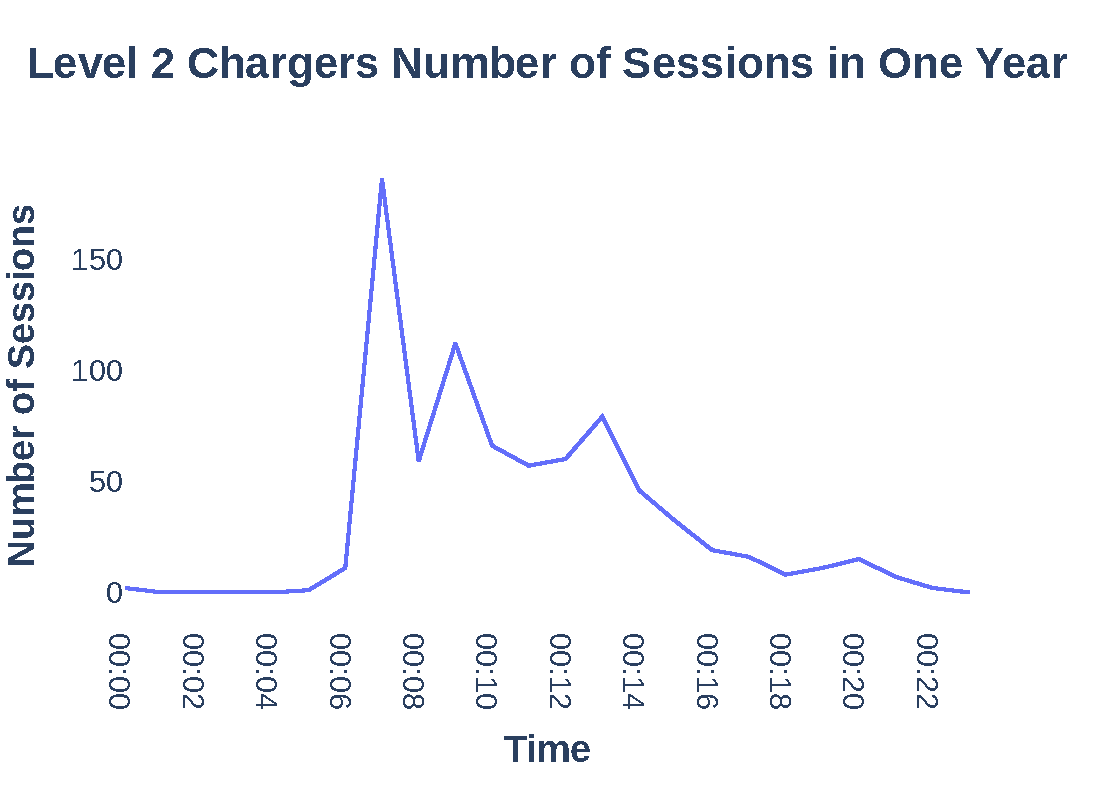
\includegraphics[width=0.9\linewidth]{Fig/Option_3/l2_avg_day_rand_poisson_1_hour_real.pdf}
\caption{\footnotesize Level 2 EV Charger Probability Density Function  Created  by Using Actual Charging Data Obtained from a SCADA System}
\label{fig:l2avgdayrandpoisson1hourpdf}
\end{figure}
\begin{figure}
\centering
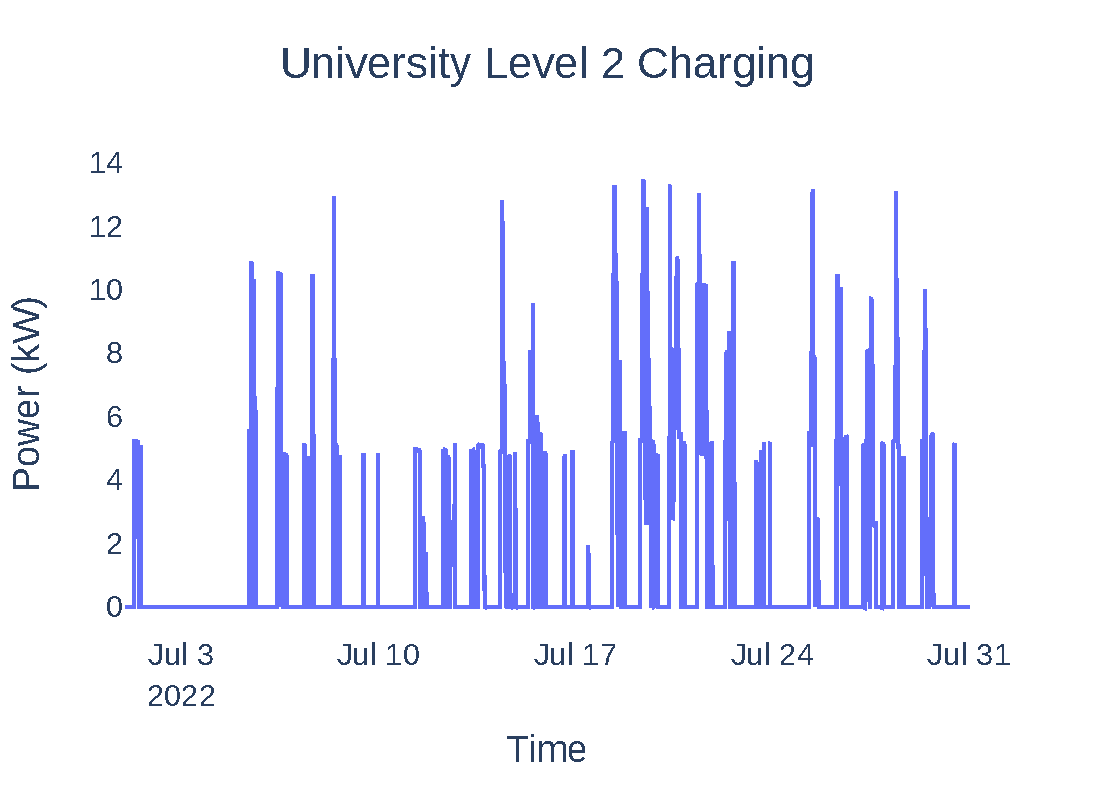
\includegraphics[width=0.9\linewidth]{Fig/Option_3/L2_short.pdf}
\caption{\footnotesize Example Level 2 Chargers Power Draw from SCADA system}
\label{fig:l2short}
\end{figure}
\begin{figure}
\centering
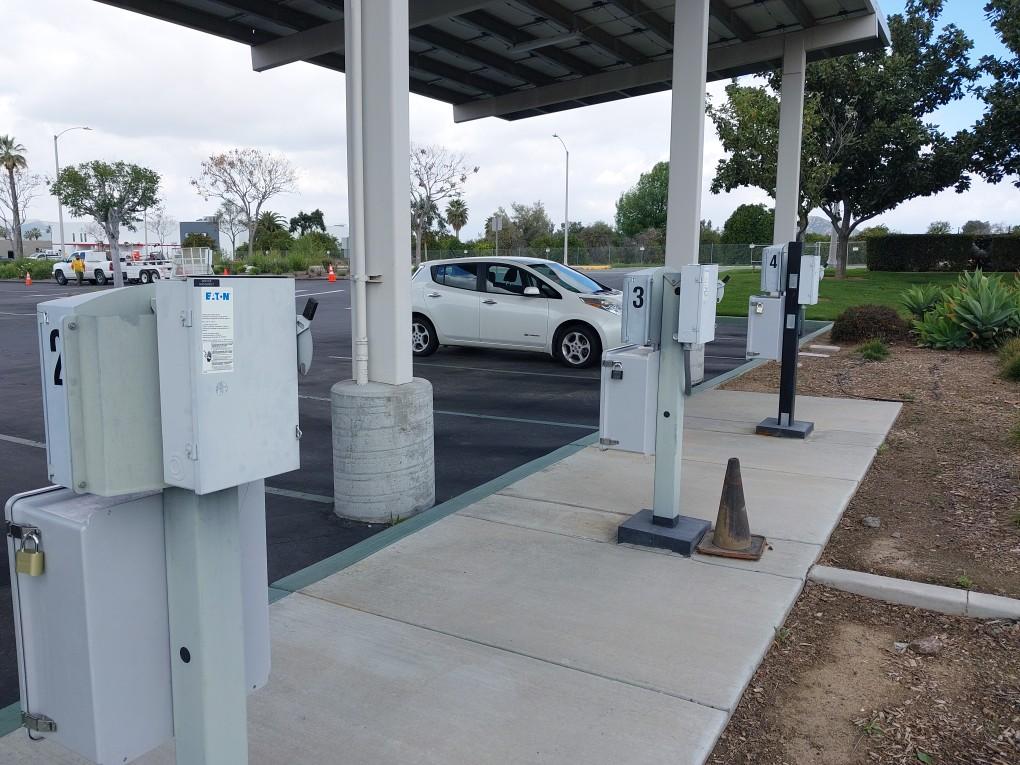
\includegraphics[width=0.9\linewidth]{Fig/Option_3/level_2_cert}
\caption{Level 2 Charging Setup}
\label{fig:level2cert}
\end{figure}

%   		However, the number of sessions and duration is reduced to X and Y for the Level 3 charger.  
%		\begin{figure}[H]
%			\centering
%			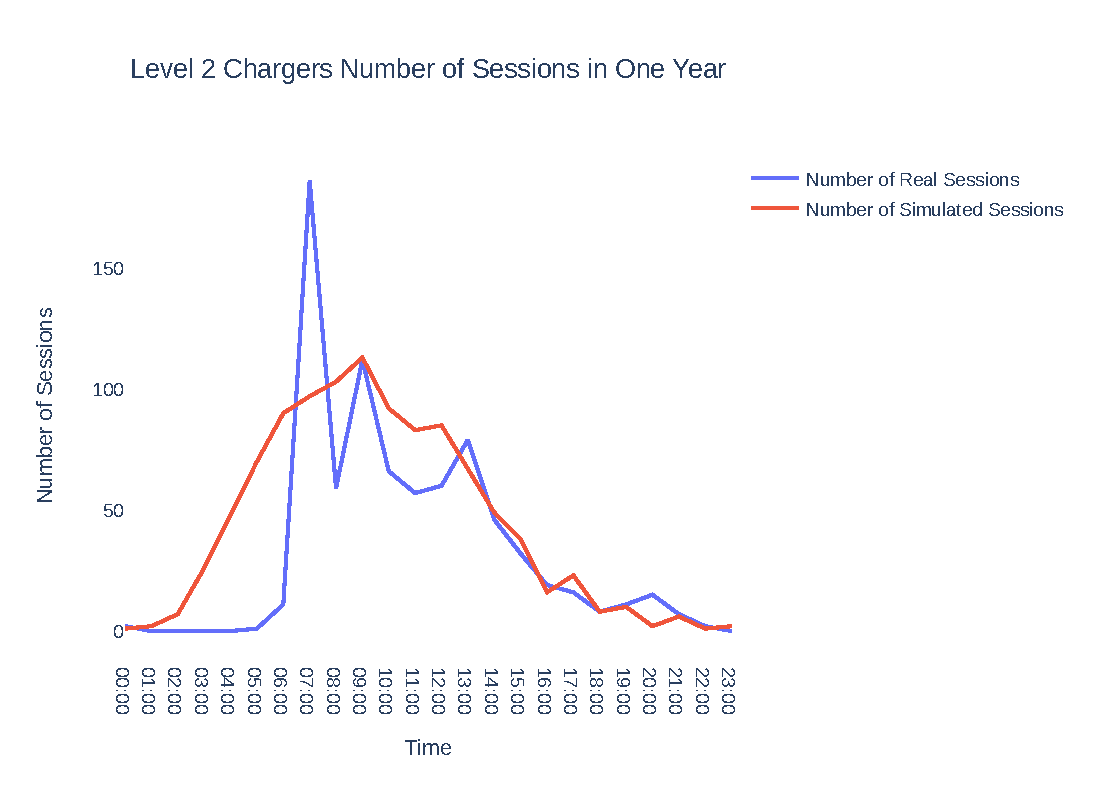
\includegraphics[width=0.9\linewidth]{Fig/l2_avg_day_rand_poisson_1_hour}
%			\caption{Number of Real and Simulated Sessions}
%			\label{fig:l2avgdayrandpoisson1hour}
%		\end{figure}
%		Historical data was collected from the Level-2 charger to determine the parameters for the Poisson random generator, following a typical daily charge pdf shown in Fig. \ref{fig:l2avgdayrandpoisson1hourpdf}, and the power output of the Level 2 chargers in Fig. \ref{fig:l2gpadpoissonjune}. After analyzing the historical data, three peak charging usually occur at $[7, 9, 13]$ with the average number of cars arriving during each peak being $[6, 2, 1]$. A mean charging time of 90 minutes is assumed. The EV random arrivals functions generate random arrival times and duration using these two parameters. The function uses numpy, a Python library, to create a Poisson random distribution with the means centered around the peak times. The random data has a seed value of 10, so every EV charging load event in the different scenarios is the same to prevent any higher demand event from being solely attributed to an outlier event from the EV charging load. The random arrivals for Level 3 charging are modeled as having three peak times: $[7, 9, 13]$, number of vehicle arrivals: $[2, 1, 1]$, and a charging mean time of 30 minutes.  
Data from the Level-2 charger SCADA system was utilized to determine the parameters for the probability density function (PDF) depicted in Fig. \ref{fig:l2avgdayrandpoisson1hourpdf}. Additionally, the power output of the Level 2 chargers is illustrated in Fig. \ref{fig:l2short}. Analysis of the historical data revealed three distinct peak charging periods occurring at 7:00, 9:00, and  13:00, respectively, with an average number of vehicle arrivals of 6, 2, and 1 during each peak. The Level 2 SCADA data is used in the Level 2 charger load simulation. The random arrivals for Level 3 charging are modeled with three peak times at 7:00, 9:00, and 13:00, with an average number of vehicle arrivals of 2, 1,  and 1, respectively. Level 3 charging has a mean charging time of 30 minutes. The EV random arrivals function uses these parameters to generate random arrival times and durations. The function employs the NumPy library\cite{NumPy}\cite{numpy_poi} in Python to create a Poisson random distribution with means centered around the peak times. To ensure consistency across different scenarios and prevent any outlier event from the EV charging load from disproportionately influencing higher demand events, a random data seed value of 10 was employed to ensure every charging event was the same. 

%		\begin{figure}[H]
%			\centering
%			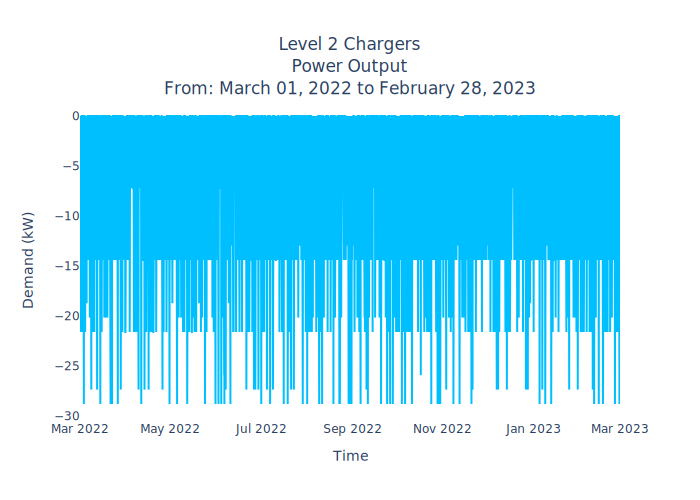
\includegraphics[width=0.9\linewidth]{Fig/ev_l2_po}
%			\caption{Level 2 Power Output}
%			\label{fig:evl2po}
%		\end{figure}
\subsection{BESS and Load-Following}
The BESS is modeled as a battery connected to a bidirectional inverter. Data generated by the control algorithm controls the BESS output. The BESS output is computed in real-time using a load-following algorithm utilizing  BESS SOC and the grid meter output. The algorithm charges the battery when excess solar power is exported to the grid and when the battery needs to be charged. Our algorithm reads the net load from the grid model and determines the amount of CO\textsubscript{2} produced during that interval. Algorithm \ref{alg:peakshavingflatrate} shows the load the following algorithm sufficient for 0 kW operation. 

%    	However,  for a TOU pricing structure, energy and demand charges are assumed to be TOU rates with no additional flat rate demands. The TOU peak shaving algorithm is presented in Equation 1 with a simple objective to minimize the amount of power the microgrid pulls from the grid while accounting for energy and demand charges. The minimization objective is accomplished by optimizing for the summation of  TOU energy ($\Delta t \boldsymbol{\alpha}^{\boldsymbol{T}} \boldsymbol{P}^G$) and the maximums TOU demands ($\max \left(\boldsymbol{\beta}^{\text {On }} \boldsymbol{P}^G\right)+\max \left(\boldsymbol{\beta}^{\text {Mid }} \boldsymbol{P}^G\right)+\max \left(\boldsymbol{\beta}^{\text {Off }} \boldsymbol{P}^G\right)$). This algorithm is further described and validated in \cite{hasan2023universal},  \cite{hasan2021comprehensive} . \\
%%		\begin{figure}
%%			\centering
%%			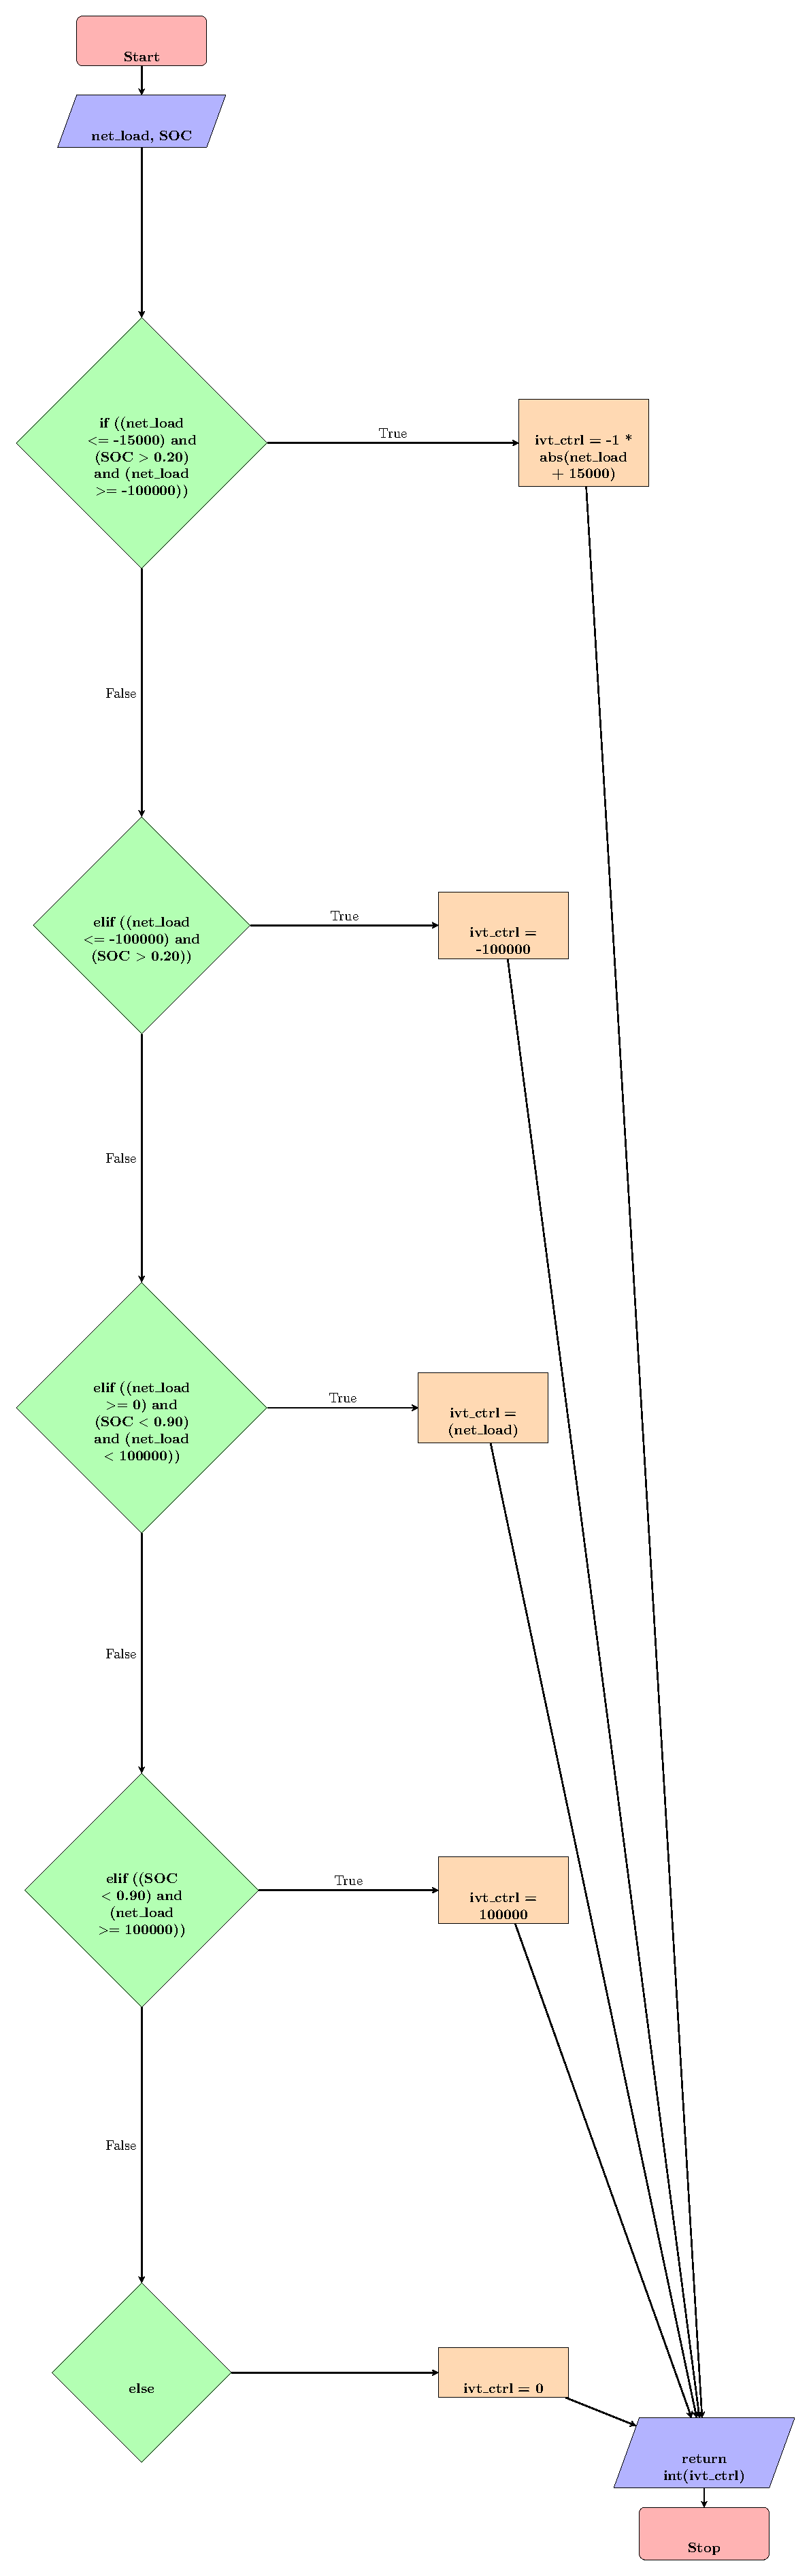
\includegraphics[width=0.7\linewidth]{Fig/peak_shaving_flat_rate}
%%			\caption{Flat Rate Peak Shaving Algorithm Flowchart}
%%			\label{fig:peakshavingflatrate}
%%		\end{figure}
%			\normalsize
%			\footnotesize
%		\begin{equation} 
%			\min f\left(\boldsymbol{P}^G\right)=\Delta t \boldsymbol{\alpha}^{\boldsymbol{T}} \boldsymbol{P}^G+\max \left(\boldsymbol{\beta}^{\text {On }} \boldsymbol{P}^G\right)+\max \left(\boldsymbol{\beta}^{\text {Mid }} \boldsymbol{P}^G\right)+\max \left(\boldsymbol{\beta}^{\text {Off }} \boldsymbol{P}^G\right)
%		\end{equation}
%		\normalsize
%		subject to
%		$$
%		\begin{aligned}
%			& E_{t+1}^B=E_t^B+P_t^B \cdot \Delta t, \forall t \in \boldsymbol{T}^{\mathbf{t o t}} \\
%			& E^{B m i n} \leq E_t^B \leq E^{B m a x}, \forall t \in \boldsymbol{T}^{\mathbf{t o t}} \\
%			& P_t^B=P_t^{B+}-P_t^{B-}, \forall t \in \boldsymbol{T}^{\text {tot }} \\
%			& 0 \leq P_t^{B+} \leq \delta_t P^{B+\max }, \forall t \in \boldsymbol{T}^{\mathbf{t o t}} \\
%			& 0 \leq P_t^{B-} \leq\left(1-\delta_t\right) P^{B-\max }, \forall t \in \boldsymbol{T}^{\mathbf{t o t}} \\
%			& 0 \leq \delta_t \leq 1, \forall t \in \boldsymbol{T}^{\mathbf{t o t}} \\
%			& P_t^{B+}=\eta^{+} P_t^{S B}, \forall t \in \boldsymbol{T}^{\mathbf{t o t}} \\
%			& P_t^S=P_t^{S B}+P_t^{S L}, \forall t \in \boldsymbol{T}^{t o t} \\
%			& P_t^L=P_t^{S L}+P_t^{B L}+P_t^G, \forall t \in \boldsymbol{T}^{\text {tot }} \\
%			& P_t^{B L}=\eta^{-} P_t^{B-}, \forall t \in \boldsymbol{T}^{t o t} \\
%			& P_t^{S L} \geq 0, \forall t \in \boldsymbol{T}^{t o t}
%		\end{aligned}
%		$$
\begin{algorithm}
net\_load, SOC $\gets$ Modelica Data Output \\
\uIf{net\_load  <=   0 kW and SOC > 20 \%  and net\_load  >=  -100 kW}{
	BESS\_inverter = -net\_load
}
\uElseIf{net\_load  <= -100 kW and SOC > 20 \%}{
	BESS\_inverter = -100 kW
}
\uElseIf{net\_load  >=  0 kW and SOC < 90 \%  and net\_load  <=  100 kW}{ 
	BESS\_inverter = net\_load
}
\uElseIf{net\_load  >=  0 kW and SOC < 90 \%  }{
	BESS\_inverter = 100 kW
}
\Else{
	BESS\_inverter = 0
}
\caption{Load-Following}
\label{alg:peakshavingflatrate}
\end{algorithm}
\begin{table*}
\caption{Simulated Scenarios of the example UCR Microgrid under Different Battery Sizes and EV Charging Demands}
\begin{tabularx}{\linewidth}{l | l}
\toprule
 Scenario &  \\
\midrule
		1  & Standard Building with no EV Chargers\\
        2 & Standard Building with Level 2 Charging\\
        3 & Standard Building with Level 2 and Level 3 Charging \\
        4 &  Microgrid Building with 100 kW Solar, 500 kWh BESS, and No EV Charging\\
        5 & Microgrid Building with 100 kW Solar, 500 kWh BESS,  and Level 2 Charging\\
        6 & Microgrid Building with 100 kW Solar, 500 kWh BESS, Level 2, and Level 3 Charging\\
        7 & Microgrid Building with 100 kW Solar, 1 MWh BESS, and Level 2 Charging\\
        8 & Microgrid Building with 100 kW Solar, 2 MWh BESS, Level 2, and Level 3 Charging\\
\bottomrule
\end{tabularx}

\normalsize
\label{tab:scenarios}
\end{table*}
\section{Results}
The charging setup in OpenModelica is modified for different layouts and scenarios, as described in Table \ref{tab:scenarios}.

Scenario 1 represents the baseline case where only the building loads, such as air conditioners, appliances, and lights, are connected to the grid. Scenario 2 represents a building installing four Level 2 EV chargers. Scenario 3 adds one Level 3 charger to the building and the Level 2 chargers. Scenario 4 is the first case that utilizes a microgrid, which includes 100 kW of solar power and 500 kWh of battery storage. This scenario demonstrates the peak-shaving capabilities of a microgrid without EV chargers, creating high demand. This can be thought of as the baseline case for the BESS microgrid. Scenarios 5, 6, 7, and 8 represent a transportation microgrid with EV chargers; the BESS capacity is varied to different sizes that include or exclude Level 3 charging to show which BESS size offers the lowest cost and the lowest CO\textsubscript{2} emissions, as well as the impact Level 3 charging has on the transportation-based microgrid.

Each scenario is run independently of the others, and the power outputs of the different components in the simulation are shown in Fig. \ref{fig:scenariospoweroutputboxplot}. Scenarios 1, 2, and 3 are constantly negative, meaning they pull power from the grid. Scenarios 3-8, on the other hand, mostly stay at zero, meaning they either export power to the grid when the BESS SOC is over 90\% or import power from the grid when it is under 20\%.

While the load-following algorithm should limit the amount of power consumed at any time to near zero kW, there are still times when the BESS cannot supply the building with power. This happens when the BESS is too depleted, and there is little to no solar power to replenish it, as shown in Figure \ref{fig:scenario3peakshaving}. The two main reasons for these events are multiple cloudy days and electrical faults. The larger the battery capacity, the less frequently the battery is depleted, and the microgrid can better weather events of low solar output. Most of the low solar power events occur during the winter months.\\
\indent Figures \ref{fig:scenariospoweroutputboxplot}, \ref{fig:0scnoutputrun2mar012022tomar312022}, and \ref{fig:4scnoutputrun2jul012022tojul312022} show box plots of the power output. Fig. \ref{fig:scenariospoweroutputboxplot} is for the entire year, while Figures \ref{fig:0scnoutputrun2mar012022tomar312022} and \ref{fig:4scnoutputrun2jul012022tojul312022} show selected months. The box plots show that all three figures' mean and 75th percentile are almost identical at 0 kW. This implies that the following load functions correctly most of the time. However, the outliers show when the BESS fails to keep the power pulled from the grid at 0 kW. Fig. \ref{fig:scenariospoweroutputboxplot} shows that Scenarios 4 - 8 have almost identical values. However, this is because the figure is maximum for the entire year. Only a few of the billing months have a solar outage long enough to cause BESS depletion that causes a demand peak almost as large as the no BESS scenario (Scenario 2).\\
\indent Just one outlier will change the demand charge for the entire billing month. In some months, the maximum demand peak of Scenario 2 and 3 is similar since they have the same load, but for most of the months, it is reduced significantly, reflected in the reduced demand charges of the building. \\ 
\indent Figures \ref{fig:scenario3peakshaving} and \ref{fig:scenario4peakshaving} demonstrate the challenges that arise when utilizing Level 3 charging compared to Level 2 charging. In Fig. \ref{fig:scenario3peakshaving}, the microgrid mostly maintains zero power consumption from the grid, occasionally exporting power to the grid with minimal imports. In Fig. \ref{fig:scenario4peakshaving}, the microgrid still maintains a mostly zero power consumption but experiences higher power imports from the grid due to battery depletion. While the demand peaks vary significantly between Level 2 and Level 3 charging, the overall energy consumption of the microgrid compared to local solar production remains similar, as shown in Table \ref{tab:gen_load_level_2_level_3}.\\

\indent The average daily CO\textsubscript{2} emissions from each scenario are shown in Fig. \ref{fig:emissionsscenariocomparison}. 
%	Scenario 2, with its increased charging events, shows about a 26\% increase in CO\textsubscript{2} emissions compared to Scenario 1. The CO\textsubscript{2} emissions from the transportation-microgrids are lower than a conventional building, even with the additional load from the EV chargers. While adding 40\% to 180\% more CO\textsubscript{2} emissions compared to a microgrid without EV charging infrastructure (Scenario 3), those CO\textsubscript{2} emissions are easily offset by charging a multitude of vehicles per day. 
Scenario 2, with its increased charging events, shows about a 26\% increase in CO\textsubscript{2} emissions compared to Scenario 1. The CO\textsubscript{2} emissions from the transportation-microgrids are lower than a conventional building, even with the additional load from the EV chargers. This case study shows that integrating a BESS coupled with peak morning charging significantly alters the characteristic emissions profile of the microgrid, deviating from the conventional duck curve paradigm. Unlike the typical afternoon peak observed in traditional duck curve scenarios, the microgrid under examination exhibits a peak demand period during the early morning. This phenomenon is attributed to the near depletion of the battery reserve, diminished solar power generation, and heightened demand for electric vehicles (EVs) during this timeframe. Table \ref{tab:emissions} shows each scenario's emissions and electric price amounts.
\begin{figure}
\centering
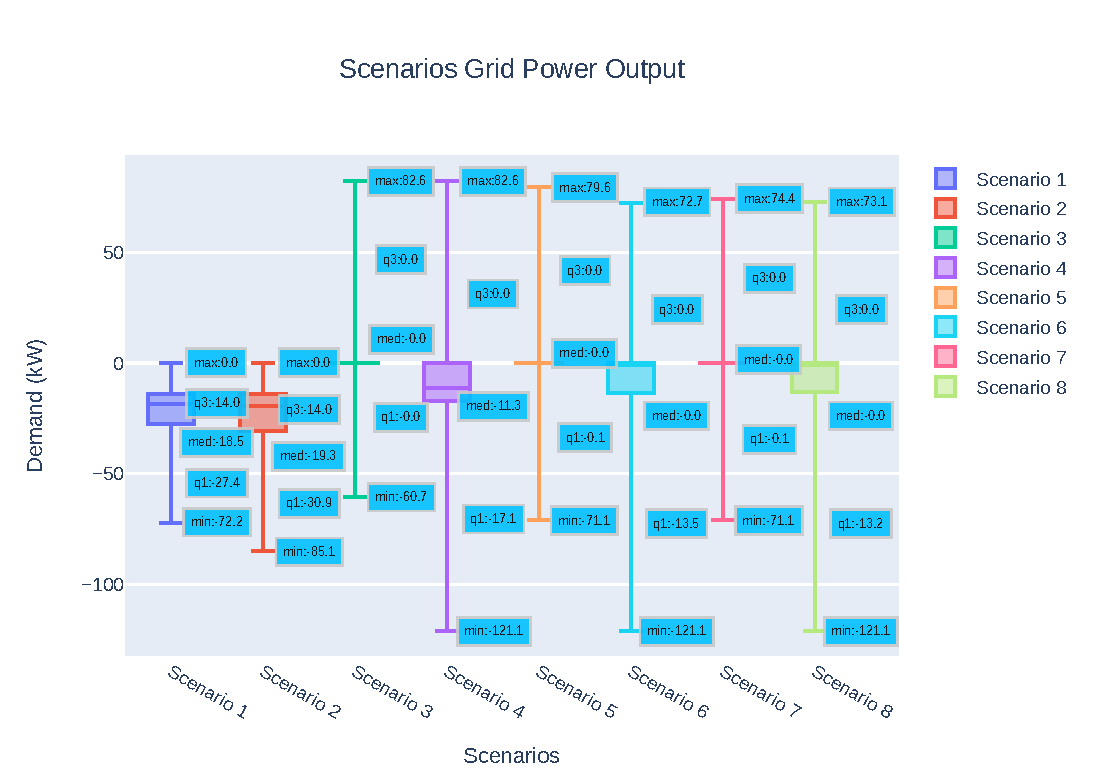
\includegraphics[width=1\linewidth]{Fig/Option_3/scenarios_power_output_boxplot}
\caption{power measured from the meter for the entire year}
\label{fig:scenariospoweroutputboxplot}
\end{figure}
\begin{figure}
\centering
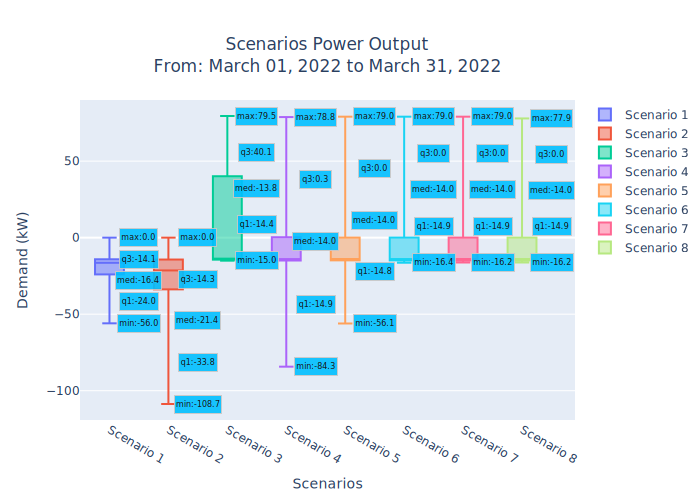
\includegraphics[width=1\linewidth]{Fig/Option_3/0_Scn_Output_Run_3_Mar_01_2022_to_Mar_31_2022}
\caption{\footnotesize  Power measured from the meter for March}
\label{fig:0scnoutputrun2mar012022tomar312022}
\end{figure}
\begin{figure}
\centering
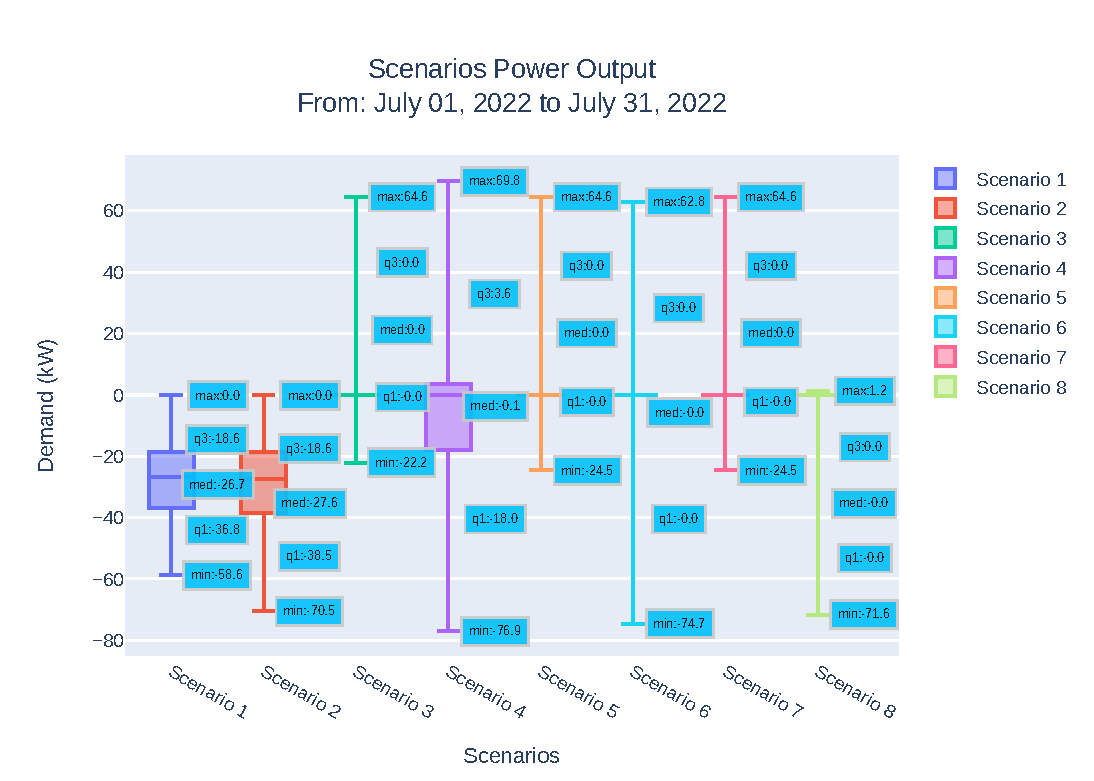
\includegraphics[width=1\linewidth]{Fig/Option_3/4_Scn_Output_Run_3_Jul_01_2022_to_Jul_31_2022}
\caption{\footnotesize  Power measured from the meter for July}
\label{fig:4scnoutputrun2jul012022tojul312022}
\end{figure}
%	\begin{figure}[H]
%		\centering
%		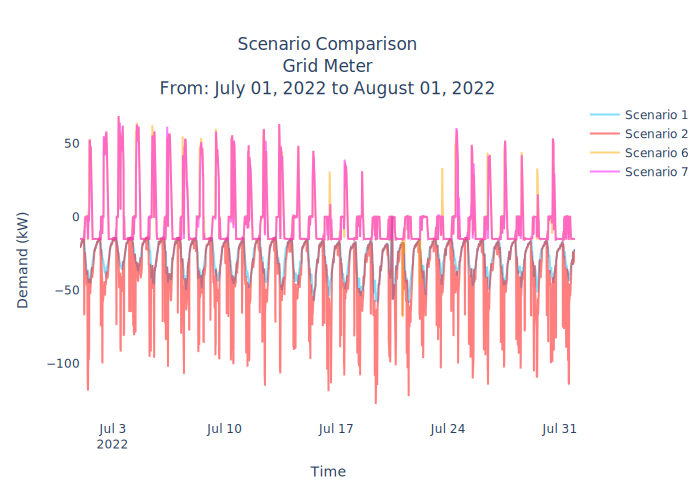
\includegraphics[width=0.9\linewidth]{Fig/net_load_scenario_comparison_summer_run_3}
%		\caption{Summer Net Load Scenario Comparison}
%		\label{fig:netloadscenariocomparisonsummer}
%	\end{figure}
\begin{figure}
\centering
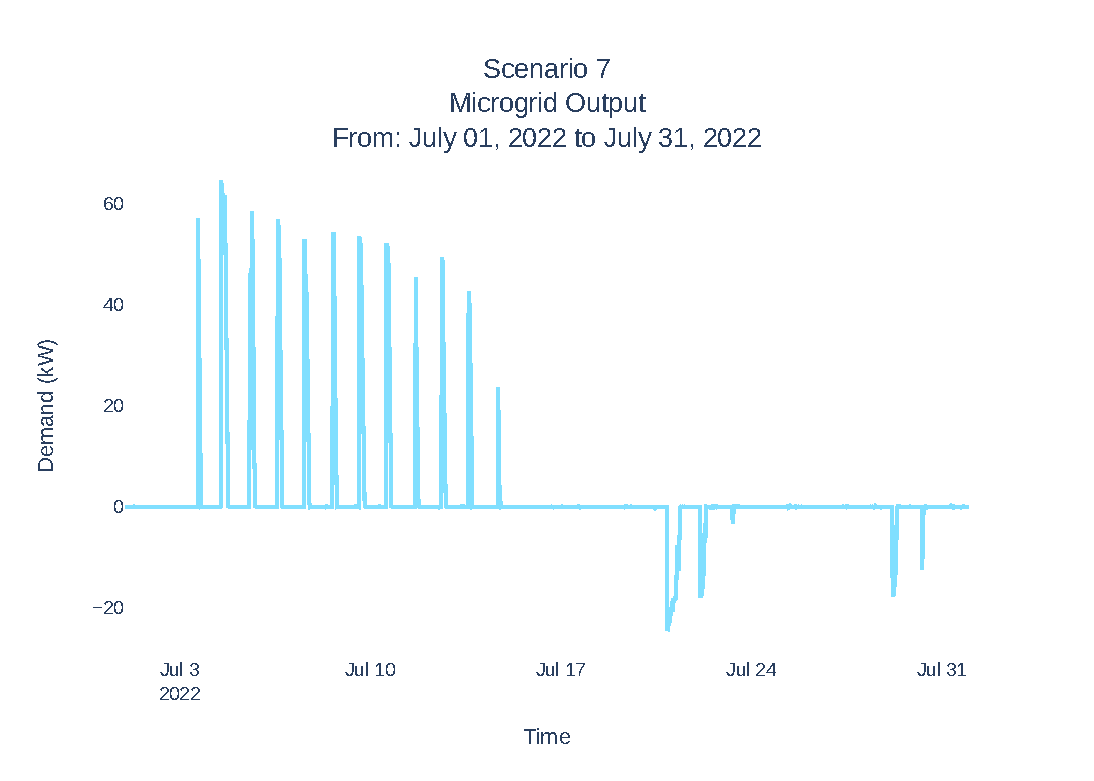
\includegraphics[width=\linewidth]{Fig/Option_3/4_Scenario_7_Run_3_Mg_Output_Jul_01_2022_to_Jul_31_2022.pdf}
\caption{\footnotesize Load Following Failures after Battery Depletion (Level 2 Charging, 1 MWh BESS)}
\label{fig:scenario3peakshaving}
\end{figure}
\begin{figure}
\centering
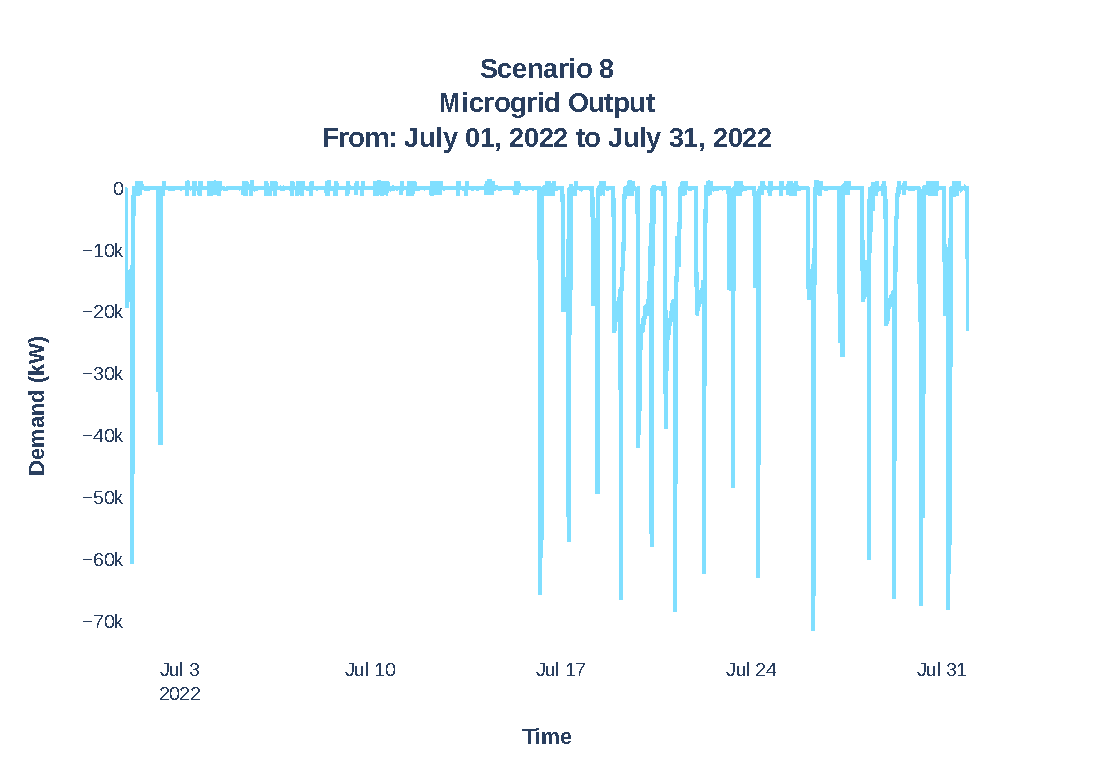
\includegraphics[width=\linewidth]{Fig/Option_3/4_Scenario_8_Run_3_Mg_Output_Jul_01_2022_to_Jul_31_2022.pdf}
\caption{\footnotesize Load Following Failures after Battery Depletion (Level 2 and Level 3 Charging, 1 MWh BESS)}
\label{fig:scenario4peakshaving}
\end{figure}
\begin{figure}
\centering
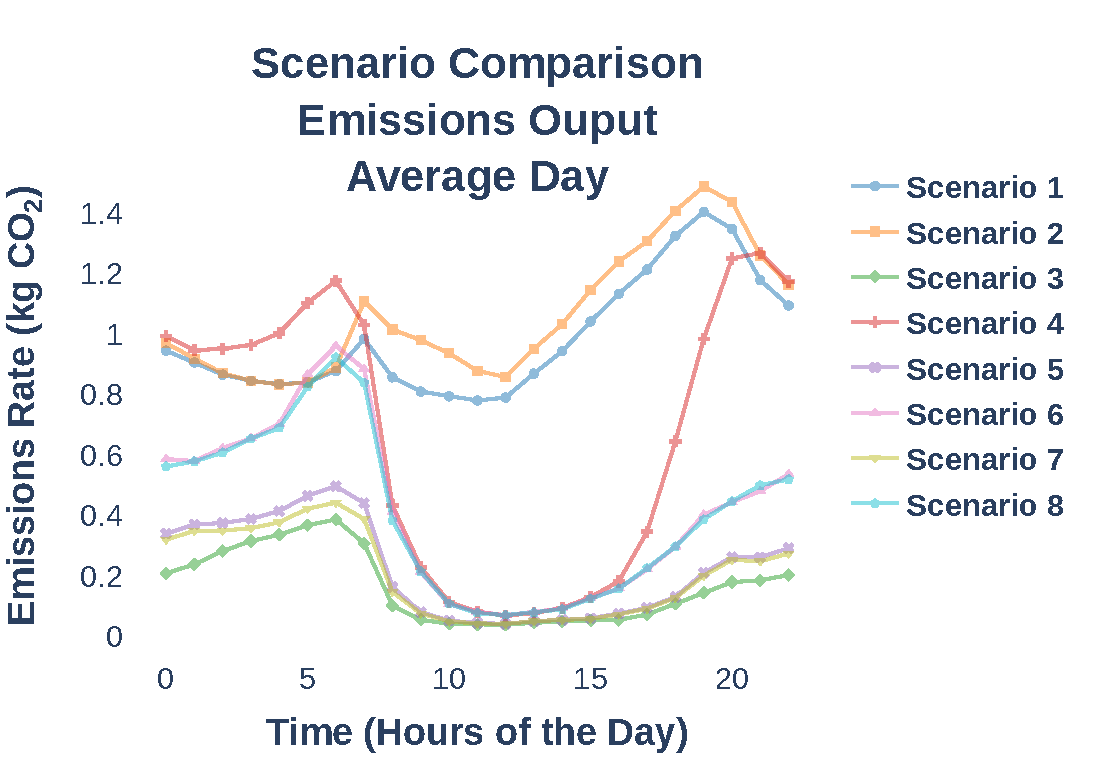
\includegraphics[width=1\linewidth]{Fig/Option_3/emissions_scenario_comparison_run_3_large_font.pdf}
\caption{\footnotesize  CO\textsubscript{2} Emissions Outputs Averages During Times of Day, using a microgrid setup}
\label{fig:emissionsscenariocomparison}
\end{figure}
\begin{table*}
\caption{Microgrid Utility Prices and CO\textsubscript{2} Emissions Output under Different Battery Sizes and EV Charging Demands}
\centering
\begin{tabular}{rrrrr}
\toprule
 Scenario &  Demand Charges (\$) &  Energy Charges (\$) &  Total Cost (\$) &  Emissions \\
\midrule
        1 &                6616 &               22736 &           29352 &         34 \\
        2 &                8196 &               24607 &           32803 &         37 \\
        3 &                3887 &                1556 &            5443 &          5 \\
        4 &               11744 &                5841 &           17585 &         23 \\
        5 &                5133 &                3256 &            8389 &          7 \\
        6 &               11329 &                8091 &           19420 &         14 \\
        7 &                5022 &                3396 &            8418 &          7 \\
        8 &               11400 &                8075 &           19475 &         14 \\
\bottomrule
\end{tabular}

\normalsize
\label{tab:emissions}
\end{table*}	
%	\begin{figure}
%		\centering
%		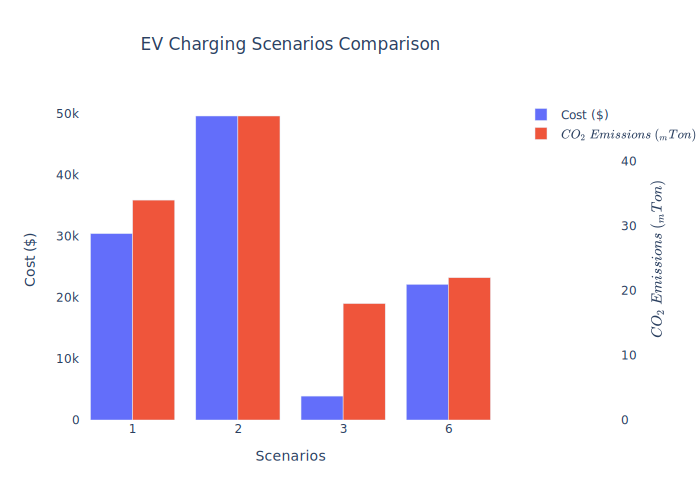
\includegraphics[width=0.9\linewidth]{Fig/mg_scene_comparison}
%		\caption{\footnotesize EV Charging Scenarios Comparison}
%		\label{fig:mgscenecomparison}
%	\end{figure}
%	\begin{figure}
%		\centering
%		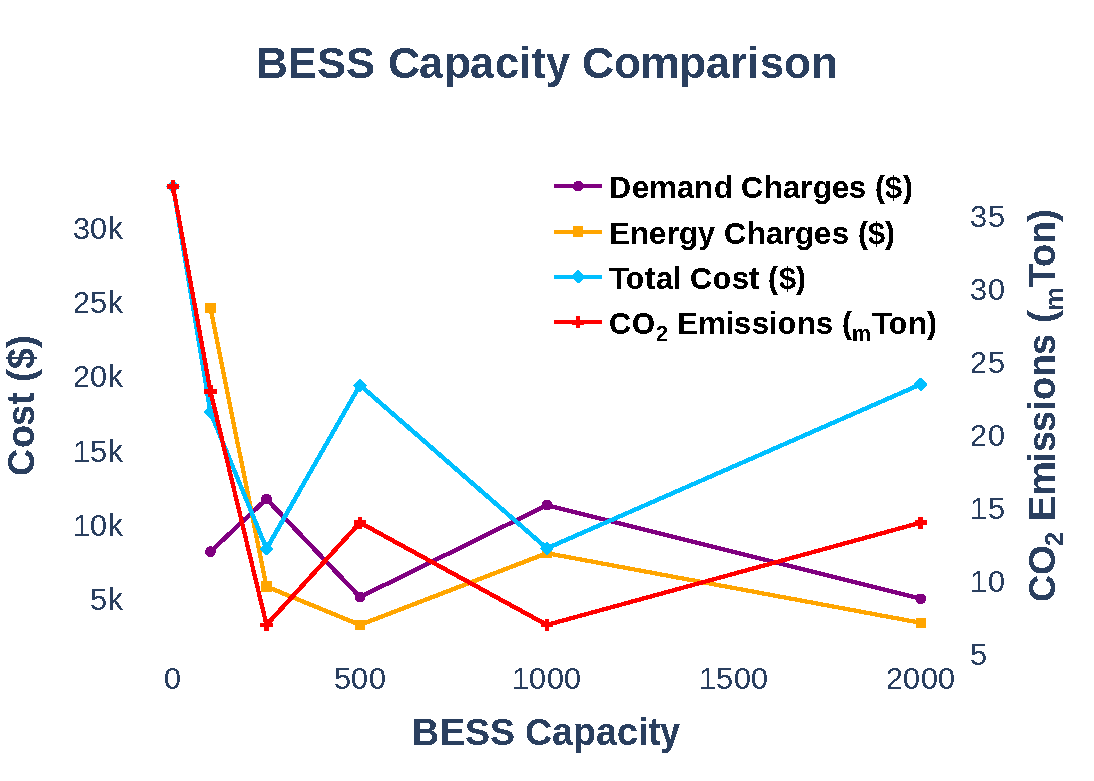
\includegraphics[width=0.9\linewidth]{Fig/Option_3/bess_capacity_comparison_large_font.pdf}
%		\caption{\footnotesize Cost and CO\textsubscript{2} Emissions for Different Battery Capacities}
%		\label{fig:besscapacitycomparison}
%	\end{figure}
\begin{table*}
\centering
\caption{Microgrid Building Power Generation \& Consumption \\ (This table determines if the renewable energy produced is sufficient to meet demand)}
\begin{tabular}{lrrrrr}
\toprule
\scriptsize Billing Month &  \scriptsize Energy Produced  (MWh) &  \scriptsize Capacity Factor \%  &  \scriptsize No EV Charging (MWh) & \scriptsize Level  2 Charging  (MWh) & \scriptsize  Level 2 \& 3 Charging  (MWh) \\
\midrule
\normalsize
Entire Interval &                 202 &                 23  &        -183 &        -198 &        -239  \\
Mar\_01\_2022 to Mar\_31\_2022 &                  22 &                 29 &         -14 &         -15 &         -19  \\ 
Apr\_01\_2022 to Apr\_30\_2022 &                  15 &                 21  &         -15 &         -16 &         -19 \\
May\_01\_2022 to May\_31\_2022 &                  12 &                 16 &         -10 &         -11 &         -14 \\
Jun\_01\_2022 to Jun\_30\_2022 &                  16 &                 23 &         -21 &         -22 &         -26  \\
Jul\_01\_2022 to Jul\_31\_2022 &                  26 &                 36   &         -21 &         -21 &         -25 \\
Aug\_01\_2022 to Aug\_31\_2022 &                  23 &                 31  &         -22 &         -24 &         -27 \\
Sep\_01\_2022 to Sep\_30\_2022 &                  20 &                 28 &         -21 &         -23 &         -26 \\
Oct\_01\_2022 to Oct\_31\_2022 &                  18 &                 24  &         -16 &         -17 &         -21 \\
Nov\_01\_2022 to Nov\_30\_2022 &                  15 &                 21 &         -12 &         -13 &         -16  \\
Dec\_01\_2022 to Dec\_31\_2022 &                  11 &                 15  &         -11 &         -12 &         -15  \\
Jan\_01\_2023 to Jan\_31\_2023 &                  10 &                 13  &          -8 &         -10 &         -13   \\
Feb\_01\_2023 to Feb\_28\_2023 &                   9 &                 14  &          -7 &          -8 &         -11\\
\bottomrule
\end{tabular}

\label{tab:gen_load_level_2_level_3}
\end{table*}	
%	\begin{table}
%		\caption{Microgrid Building Power Consumption}
%		\tiny
%		\centering
%		\begin{tabular}{lrrr}
\toprule
             Billing Month &  No EV Charging &  Level  2 Charging &  Level 2 \& 3 Charging\\
\midrule
           Entire Interval &        -183 &        -198 &        -239  \\
Mar\_01\_2022 to Mar\_31\_2022 &         -14 &         -15 &         -19  \\
Apr\_01\_2022 to Apr\_30\_2022 &         -15 &         -16 &         -19  \\
May\_01\_2022 to May\_31\_2022 &         -10 &         -11 &         -14  \\
Jun\_01\_2022 to Jun\_30\_2022 &         -21 &         -22 &         -26  \\
Jul\_01\_2022 to Jul\_31\_2022 &         -21 &         -21 &         -25 \\
Aug\_01\_2022 to Aug\_31\_2022 &         -22 &         -24 &         -27 \\
Sep\_01\_2022 to Sep\_30\_2022 &         -21 &         -23 &         -26\\
Oct\_01\_2022 to Oct\_31\_2022 &         -16 &         -17 &         -21  \\
Nov\_01\_2022 to Nov\_30\_2022 &         -12 &         -13 &         -16 \\
Dec\_01\_2022 to Dec\_31\_2022 &         -11 &         -12 &         -15  \\
Jan\_01\_2023 to Jan\_31\_2023 &          -8 &         -10 &         -13  \\
Feb\_01\_2023 to Feb\_28\_2023 &          -7 &          -8 &         -11 \\
\bottomrule
\end{tabular}

%		\normalsize
%		\label{tab:load_level_2_level_3.tex}
%	\end{table}	
%	\begin{table}
%		\caption{Solar Power Production}
%		\tiny
%		\centering
%		\begin{tabular}{lrr}
\toprule
             Billing Month &  Energy Produced  (MWh) &  Capacity Factor \% \\
\midrule
           Entire Interval &                 202 &                 23 \\
Mar\_01\_2022 to Mar\_31\_2022 &                  22 &                 29 \\
Apr\_01\_2022 to Apr\_30\_2022 &                  15 &                 21 \\
May\_01\_2022 to May\_31\_2022 &                  12 &                 16 \\
Jun\_01\_2022 to Jun\_30\_2022 &                  16 &                 23 \\
Jul\_01\_2022 to Jul\_31\_2022 &                  26 &                 36 \\
Aug\_01\_2022 to Aug\_31\_2022 &                  23 &                 31 \\
Sep\_01\_2022 to Sep\_30\_2022 &                  20 &                 28 \\
Oct\_01\_2022 to Oct\_31\_2022 &                  18 &                 24 \\
Nov\_01\_2022 to Nov\_30\_2022 &                  15 &                 21 \\
Dec\_01\_2022 to Dec\_31\_2022 &                  11 &                 15 \\
Jan\_01\_2023 to Jan\_31\_2023 &                  10 &                 13 \\
Feb\_01\_2023 to Feb\_28\_2023 &                   9 &                 14 \\
\bottomrule
\end{tabular}

%		\normalsize
%		\label{tab:mg_gen_level_2_level_3}
%	\end{table}	
\begin{table*}[t]
\caption{Riverside Public Utility Commercial Demand Rate \cite{rpu_rate}}
\centering
\begin{tabular}{|l|c|r|r|r|r|r|}
	\hline \multicolumn{2}{|c|}{} & \multicolumn{5}{|c|}{ Per Meter, Per Month Effective January 1, } \\
	\hline & & 2024 & \multicolumn{1}{|c|}{2025} & \multicolumn{1}{|c|}{2026} & \multicolumn{1}{c|}{2027} & \multicolumn{1}{c|}{2028} \\
	\hline Customer Charge & Flat Charge & $\$ 22.10$ & $\$ 22.10$ & $\$ 22.10$ & $\$ 22.10$ & $\$ 22.10$ \\
	\hline Reliability Charge & Flat Charge & $\$ 90.00$ & $\$ 90.00$ & $\$ 90.00$ & $\$ 90.00$ & $\$ 90.00$ \\
	\hline Network Access Charge & \$ Per kW & $\$ 1.75$ & $\$ 1.75$ & $\$ 1.75$ & $\$ 1.75$ & $\$ 1.75$ \\
	\hline Demand Charge & \begin{tabular}{c} 
		First 15 kW or less of billing \\
		demand, flat charge
	\end{tabular} & $\$ 160.95$ & $\$ 160.95$ & $\$ 160.95$ & $\$ 160.95$ & $\$ 160.95$ \\
	\hline Demand Charge & \begin{tabular}{c} 
		All excess kW of billing \\
		demand, per kW
	\end{tabular} & $\$ 10.73$ & $\$ 10.73$ & $\$ 10.73$ & $\$ 10.73$ & $\$ 10.73$ \\
	\hline
\end{tabular}
%\begin{tabular}{|l|c|r|r|r|r|r|}
%\hline \multicolumn{2}{|c|}{} & \multicolumn{5}{c|}{ Per Meter, Per Month Effective January 1,} \\
%\hline & Flat Charge & 2024 & \multicolumn{1}{|c|}{2025} & \multicolumn{1}{|c|}{2026} & \multicolumn{1}{|c|}{2027} & 2028 \\
%\hline Customer Charge & Flat Charge & $\$ 22.10$ & $\$ 22.10$ & $\$ 22.10$ & $\$ 22.10$ & $\$ 22.10$ \\
%\hline Reliability Charge & $\$$ Per kW & $\$ 1.75$ & $\$ 1.75$ & $\$ 1.75$ & $\$ 1.75$ & $\$ 1.75$ \\
%\hline Network Access Charge & \begin{tabular}{c} 
%First 15 kW or less of billing \\
%demand, flat charge
%\end{tabular} & $\$ 160.95$ & $\$ 160.95$ & $\$ 160.95$ & $\$ 160.95$ & $\$ 160.95$ \\
%\hline Demand Charge & \begin{tabular}{c} 
%All excess kW of billing \\
%demand, per kW
%\end{tabular} & $\$ 10.73$ & $\$ 10.73$ & $\$ 10.73$ & $\$ 10.73$ & $\$ 10.73$ \\
%\hline Demand Charge & & $\$ 90.00$ & $\$ 90.00$ & $\$ 90.00$ \\
%\hline
%\end{tabular}

\normalsize
\label{tab:rpu_demand}
\end{table*}	
\begin{table*}[t]
\caption{Riverside Public Utility Commercial Energy Rate \cite{rpu_rate} \\ Note: The solar surplus rate to sell electricity to the grid is \$0.076 per kWh \cite{rpu_nem}}
\centering
\begin{tabular}{|c|c|c|c|c|c|c|}
	\hline \multicolumn{2}{|c|}{ Per kWh Effective January 1, } &  \multicolumn{5}{|c|}{ }  \\
	\hline & & 2024 & 2025 & 2026 & 2027 & 2028 \\
	\hline Tier 1 & $0-30,000 \mathrm{kWh}$ & $\$ 0.1242$ & $\$ 0.1242$ & $\$ 0.1242$ & $\$ 0.1242$ & $\$ 0.1242$ \\
	\hline Tier 2 & Over 30,000 kWh, per kWh & $\$ 0.1360$ & $\$ 0.1360$ & $\$ 0.1360$ & $\$ 0.1360$ & $\$ 0.1360$ \\
	\hline
\end{tabular}
\normalsize
\label{tab:rpu_energy}
\end{table*}	
\section{Conclusions}
Transportation microgrids have emerged as a compelling solution for mitigating the electrical costs and emission levels associated with EV charging infrastructure. A comprehensive analysis of various scenarios reveals significant economic and environmental benefits of transportation microgrids compared to conventional systems, as depicted in  Table \ref{tab:emissions}. For transportation-microgrid systems using a load-following algorithm, the estimated annual savings range is similar at around \$23,000 to \$24,000 for our case study, even with the additional demand from EV chargers. This implies that load-following transportation microgrids provide the same amount of savings even with varying demand and a sufficiently large BESS. The cost of demand and the cost of energy saved follow the same trend as the total cost, with the overall amount of savings being similar, \$3,000 and \$21,000, respectively, which is calculated from the commercial utility rate shown in Tables \ref{tab:rpu_demand}, \ref{tab:rpu_energy}.
Furthermore, load-following transportation-microgrids can reduce CO\textsubscript{2} emissions by 67\% to 85\%, approximately 30 tons of CO\textsubscript{2} in our case. It is important to note that while the scenarios show similar reductions in electricity prices and CO\textsubscript{2} emissions, users are strongly incentivized to acquire additional clean energy sources (solar and wind), especially when adding a Level 3 fast charger. At the same time, a couple of Level 2 chargers do not heavily strain an office building. The solar surplus rates make low CO\textsubscript{2} emission load-following more economically viable compared to just peak-shaving \cite{rpu_nem}. BESS reduces the energy pulled from the grid rather than saving up energy to address a couple of peak cases in a month.

It is important to note that increasing the battery capacity does not necessarily guarantee improved microgrid performance. Addressing the most challenging solar power outages requires a significant increase in battery capacity while providing only marginal CO\textsubscript{2} and cost savings in return. Also, extra capacity is not very useful for CO\textsubscript{2} emissions reductions without adding extra solar power to charge the battery during daylight hours completely. Lastly, any sensible microgrid planning requires addressing three key parameters: clean energy generation, energy storage, and load management. Doing only two of the three creates situations where the microgrid alone cannot power the building.
\section{Future Work}
Future research will explore different, more advanced control strategies to optimize the electric costs and CO\textsubscript{2} emissions of the transportation-microgrid. These strategies will include electric vehicle load allocation during high peak times, maximizing the use of the clean energy produced by the solar panels, and minimizing the power drawn from the grid during high CO\textsubscript{2} times. The effects of the new net energy metering policy in California on the value of the BESS system will also be assessed. The impact of different time-of-use (TOU) rates in California on electric costs and CO\textsubscript{2} emissions will be analyzed.


		%		\nocite{*}
		\bibliographystyle{IEEEtran}
		\bibliography{cite}
	
\end{document}
